\chapter{The Technological War}

\begin{quotation}
\textit{There are at least two kinds of games. One should be called finite, the other infinite. A finite game is played for the purpose of winning, an infinite game for the purpose of continuing the game.}
\newline
--James P. Carse, \textit{Finite and Infinite Games}
\end{quotation}

The United States is at war. Whether we consider this to be the Protracted Conflict initiated in 1917 by the Bolsheviks or something new brought about by the march of technology, the war cannot be escaped. The field of engagement is not everywhere bloody. Except for financial sacrifices, many citizens of the West and subjects of Communism may be unaware of the conflict until the decisive moment, if it ever comes, is upon them. For all that, the dynamic Technological War is most real, and we must understand its nature, for it is decisive. Our very survival depends on our constantly winning this battle.

The Technological War has been raging since World War II. That war marked the end of the era in which decisive military power grew exclusively from the products of the original Industrial Revolution. In the new era, power grows largely -- sometimes exclusively -- from products based on applied science.

The Technological War is dynamic. There are dramatic peaks in activities as rates of change suddenly accelerate. The theater of operations can change in bewildering ways: recent (1989) events in Europe are a prime example. Ruling classes come and go, alliances are made and dissolved; but the Technological War remains. For the West, the Technological War is an infinite game; victory in one battle, or in an entire theater of conflict, does not end the conflict.

The Technological War is seemingly impersonal because of its new and unexpected sources of change and its global impact. Even so, the Technological War, like all conflicts, is driven by human ingenuity responding to basic challenges and aspirations.

For many years the most basic challenge of the Technological War has been the threat to U.S. security caused by the enmity of the Soviet Union, specifically a small group within the ruling elite of the U.S.S.R. That group within the nomenklatura\footnote{In the first edition of this work and in other places Stefan Possony referred to a secret Soviet group which he called "the Brotherhood", and which in some ways corresponded to what we now know is the \textit{nomenklatura}.} deliberately chose the U.S. as its enemy after the close of World War II, and renewed the Protracted Conflict against the rest of the world. That conflict has lasted for over seventy years.

The true nature of the Soviet nomenklatura is not fully understood in the West even today. As a first approximation, they may be thought of as the "state engineers" whose emergence under socialism was predicted by Bakunin, and who were first described in popular literature in Milorad Djilas's The New Class. This privileged political-scientific class was the actual government of the U.S.S.R. It arose during the Stalinist purges of the 30's, gained strength shortly after World War II, and consolidated its hold on the U.S.S.R. from the time of Stalin's death until the rise of Gorbachev.

The nomenklatura were the true owners of the U.S.S.R., for not only was the population at large excluded from the political process (except for ritualistic purposes), but also the rank and file of the Communist Party, some 18 million in number, were reduced to executors of the nomenklatura's will. The nomenklatura held the Soviet Union in ownership every whit as much as had feudal landlords; it's position can best be given in the words of Karl Marx, who spoke of the post-1830 monarchy in France as " 'a company for the exploitation of the French national wealth,' of which the king was the director, and whose dividends were distributed among the ministers, parliamentary deputies, and 240,000 enfranchised citizens."

nomenklatura has two meanings: a list of the most important offices, appointment to which requires approval by the Secretariat; and the roster of the personnel who either hold those offices or are eligible for promotion to them. The numbers and names of the nomenklatura remain state secrets. In 1989 Esther Dyson was shown a copy of the Leningrad edition for 1987: a small red book consisting of about 5,000 names and addresses, with no title other than a document number and date.

Although the nomenklatura exists within the Soviet Union, it is independent of the nation in that it owes no allegiance to the country or the people; its major goal, like that of many oligarchies, is to retain its power and privileges.

This power structure has undergone dramatic changes in the Gorbachev era. It has not been abolished, and it is unlikely that it will be abolished in any short period of time. Gorbachev's official view is that the basic structure of the U.S.S.R. is sound, as was Lenin's view of the world situation; the Revolution was betrayed, but the Marxist analysis of history remains sound. In today's Soviet Union the old nomenklatura is the enemy of \textit{glasnost} and \textit{perestroika}, and must be replaced. The result is likely to be faces among the nomenklatura, and a new basis for its selection -- possibly a structure independent of and antithetical to the Communist Party. Even so, the phenomenon will remain, nor should anyone familiar with political history be surprised by that. Michels's Iron Law Of Oligarchy was written well before the Russian Revolution. Replacement of the nomenklatura would require fundamental changes in Soviet economic organization and structure, and so far those are not only not contemplated, but vigorously denounced by Gorbachev as well as by his enemies within the Party.

Thus, despite changes in Soviet structure, the basic conflict remains; and so does the Technological War. Indeed, \textit{glasnost} and \textit{perestroika} , by allowing the new Soviet leadership to abandon obsolete weapons systems, can release new resources which can be committed to the struggle. Military commanders are usually reluctant to reduce the numbers of troops they command; but in fact in the Technological War it is often better to have smaller numbers of highly effective forces than to use one's scarce technical resources to maintain obsolete equipment. For all the talk of a new era in the Cold War, the U.S.S.R. has not noticeably slowed its production of modern weapons, and is not likely to.

In addition to the Soviet threat, there is a second challenge: the threat to the U.S. economy from our erstwhile allies, who, under the shelter of the U.S. military umbrella, have exploited technology to challenge U.S. economic leadership. While purely commercial competition is outside the scope of this book, there is a strong interaction between military and economic national technological strategies. A rational strategy of technology will not neglect the means for expanding the technological base from which military technology is derived. We will return to this point later.

During the 1990's, the major conflict will be between the United States and the U.S.S.R. The natures of both technology and the enemy dictate that this will a be state of Technological War. For all the Gorbachev reforms, the U.S.S.R. is a power-oriented dictatorship, whose official doctrine is Communism: That is, a chiliastic movement which claims inevitable dominance over the entire earth. It is not necessary for all of the individual leaders of the U.S.S.R. to be true believers in this doctrine, and in fact most may not. Since the Soviet Union is a dictatorship, the usual dynamics of dictatorship apply.

The government of the Soviet Union is divided among the Army, KGB, and Party. The Party and KGB appear to be under the near total domination of the nomenklatura. The Army may not be, but military promotions are largely under the control of the Party and therefore the nomenklatura. The relation between Gorbachev and the nomenklatura is also unclear. One thing is certain: \textit{glasnost} and \textit{perestroika} cannot be implemented without using the existing power structure, and that includes the nomenklatura.

One fundamental fact of dictatorship is that losing factions within its ruling structure forever lose their positions and power. They may retain their lives -- the nomenklatura generally do -- but they retain little else, and sometimes they do not survive. Thus, such rulers, whether sincere or cynical, have a powerful incentive to conform to the official ideology or line of the top man or group. Moreover, they compete with each other for power. If a powerful faction counsels aggressive expansion -- whether out of sincere belief in the ideology, because expansion creates more opportunities for advancement, or because it expects aggression to prop up a tottering regime -- failure is the only way through which its influence will be reduced. Every successful aggressive action increases the influence of those who counsel aggression.

If aggressive moves encounter stern opposition, so that the ruling faction is not only not rewarded for its expansionist policies, but finds its national power decreased, changes in the official policy may take place. Such failures, consequent punishment, and resultant troubles for the dictatorship may serve to place in power a more cautious group dedicated to defense of the empire and the status quo.

\begin{mdframed}[backgroundcolor=black!10]
This was dramatically illustrated by the Soviet failure in Afghanistan.
\end{mdframed}

It is possible that the nomenklatura, faced with rising opposition from both ethnic minorities and even the Russian people, has veered its policy toward one of imperial defense. If so, this will mark an important turning point in history; but we cannot bet the survival of freedom on what may be a temporary policy shift based largely on the life of one man.

Moreover, if there has been a change in policy, it is due largely to the failure of the previous leaders to induce the United States to abandon the conflict entirely. Nearly twenty years ago we argued that the best way to change Soviet policy was to negotiate from strength; we believe the Reagan era has proved that.

There have been profound changes in Soviet leadership and policy since we wrote the first edition of this book. Much of the Soviet leadership has become disillusioned with the inevitability of world victory. At the same time, there is no ideological justification to the rule of the Party -- and behind that the nomenklatura -- except Communism.

\textit{glasnost} and \textit{perestroika} may be genuine; they may even work; but these changes will not and cannot remove all the incentives for expansionism, particular if expansion looks easy.

Moreover, aggressive actions may occur because of internal pressures, especially in a period when faith in Communism as an ideological system is declining, and it is possible, although unlikely, that aggressive initiatives will be taken by non-Communist states.

The international situation is complex; and despite all complications the U.S.S.R. is the single most important and strongest opponent of the United States. If the USSR leadership believes it can eliminate the United States, the temptation to do that will be severe. Consequently, American strategists must primarily be concerned with Soviet strategy and the threat posed by the U.S.S.R.\footnote{Since we wrote this in 1968-69, the Soviets have invaded Czechoslovakia to consolidate the Empire's power there; invaded Afghanistan; placed tens of divisions on the Chinese border; interfered in the Middle East; used Cuban mercenaries to destabilize a great part of Africa; induced the Communist regime in Poland to enslave its own working class; and established a beachhead on this continent in Nicaragua. Is further evidence of Soviet aggressive tendencies needed?}

This does not mean that the economic threat to the U.S. technological base can be neglected. Other nations pursue an aggressive strategy of technological competition, often guided, as with the Japanese Ministry of Trade and Industry, from the highest government levels. International technological competition can sometimes reach levels best described as economic warfare, and the outcomes of these competitive struggles can have surprisingly long range effects on the decisive military Technological War.

The nature of technology also dictates that there will be conflict. This will be discussed in greater detail in later chapters. For the moment, we can say that although technology can and should be driven by an active strategy, there is also a sense in which technology flows on without regard for human intentions, and each technological breakthrough offers the possibility for decisive advantages to the side that first exploits it. Such advantages will be fleeting, for although the weaker side does not have weapons based on the new technology yet, it is certain that it will have them in the near future. In such circumstances, failure to exploit the capability advantage is treason to the Communist cause.

It must be emphasized that to the committed Communist, there are no ideological reasons for not exploiting advantages over the capitalists. The only possible objections are operational. No communist can admit that a capitalist government is legitimate; thus there can be no "mercy" to a vulnerable capitalist regime.

Therefore, capability combines with ideology to produce a powerful effect on intentions, which, be they ever so pure before the advantage was obtained, cannot fail to change with the increasing capabilities: if capabilities grow, intentions become more ambitious.

Thus, it is futile and dangerous to base modern strategy on an analysis of the intentions of the enemy. The modern strategist must be concerned with the present and future capabilities of his opponent, not with hopes and dreams about his goals. The dynamics of dictatorship provide a continuing source of ambitious advisors who will counsel the rulers of the Soviet Union toward aggressive action, and only through continuous engagement in the Technological War can the United States ensure peace and survival.

Because the goals of the United States and the U.S.S.R. are asymmetric, the strategies each employ in the Technological War necessarily are different. The United States is dedicated to a strategy of stability. We are a stabilizing rather than a disturbing power and our goal is preserving the status quo and the balance of power rather than seeking conquest and the final solution to the problems of international conflict through occupation or extermination of all opponents. In a word, the U.S. sees the Technological War as an infinite game, one played for the sake of continuing to play, rather than for the sake of "victory" in the narrow sense.

The U.S.S.R. is expansionist; aggressive; a disturber power which officially states that the only true peace is that of world Communism. Marxist theory would make the Technological War a finite game, to be ended with a clean win.

The United States has conceded the initiative in the Protracted Conflict, and is to a great extent bound to a policy of reacting to Communist advances, rather than seeking the initiative in undermining Communist power. Because we have conceded the initiative in the phase of the Protracted Conflict which deals with control of territory and people\footnote{Robert Strausz-Hupe et al, Protracted Conflict (New York: Harper 1969); Stefan T. Possony, A Century of Conflict, 5th ed. (Chicago: Regnery, 1969); Richard Pipes, Survival Is Not Enough (New York: Simon and Schuster Touchstone Books, 1986)}, we must not abandon the initiative in the Technological War. We are engaged in a war, not a race, although it may appear to be a race to many of us. But it is a race in which we must stay ahead, because if we ever fall  behind, the opponent will blow up the bridges before our runners can cross them.

Given the opportunity, the Soviets will deny us access to the tools of the Technological War exactly as they have denied access to their territory, which they call the "peace zone" in distinction to the rest of the world which is the "war zone". If we are to be on the defensive in the Protracted Conflict, survival demands that we retain the initiative and advantage in the Technological War. We know that U.S. supremacy does not bring on global war, let alone a war of conquest; we held an absolute mastery during our nuclear monopoly. We can be certain that the Soviets would not be passive were they to gain supremacy.

The Technological War is the decisive struggle in the Protracted Conflict. Victory in the Technological War gives supremacy in all other phases of the conflict, to be exploited either by thermonuclear annihilation of the opponent, or simply demanding and obtaining his surrender. The Technological War creates the resources to be employed in all other parts of the Protracted Conflict. It governs the range of strategies that can be adapted in actual or hot war. Without the proper and superior technology our strategy of deterrence would be meaningless. Without technological advantages, we could never fight and win a small war thousands of miles from our homeland, or prevent the occupation of Europe and Japan.

Up to the present moment, technological warfare has largely been confined to pre-hot war conflict. It has been a silent and apparently peaceful war, and engagement in the Technological War is generally compatible with the strong desires of most of our people for "peace". The temporary winner of the Technological War can, if he chooses, preserve peace and order, act as a stabilizer of international affairs, and prevent shooting wars -- continue the Technological War as an infinite game.

There could be a different outcome. If the side possessing a decisive advantage sees the game as finite, the victor can choose to end the game on his own terms. The loser has no choice but to accept the conditions of the victor, or to engage in a shooting war which he has already lost.

Technological War can be carried on simultaneously with any other forms of military conflict, diplomatic maneuvers, peace offensives, trade agreements, detente, and debacle. It is the source of the advanced weapons and equipment for use in all forms of warfare. It renders cold war activities credible and effective. Technological warfare combined with psychosocial operations can lead to a position of strategic dominance.

This new form of warfare has its roots in the past, but it is a product of the current environment. World War II was the last war of industrial power and mobilization, but it was also the first war of applied science. The new war is one of the directed use of science. The manner of its use is shown by the changing nature of warfare. Wars of the past were wars of attrition of the military power which was a shield to the civilian population and the will to resist. The new technology has created weapons to be applied directly and suddenly to the national will, soon with the speed of light.

\section{Definition of Technological Warfare}
    
Technological warfare is the direct and purposeful application of the national technological base\footnote{We define as technological base the sum total of resources needed to produce and constantly modernize the tools of war and peace. Those resources include scientists, inventors, engineers, laboratories, laboratory equipment, funds, information flow, incentives, etc., as well as industry and the economy as a whole, which we do not discuss in this book.} and of specific advances generated by that base to attain strategic and tactical objectives. It is employed in concert with other forms of national power. The aims of this kind of warfare, as of all forms of warfare, are to enforce the national will on enemy powers; to cause them to modify their goals, strategies, tactics, and operations; to attain a position of security or dominance which assists or supports other forms of conflict techniques; to promote and capitalize on advances in technology to reach superior military power; to prevent open warfare; and to allow the arts of peace to flourish in order to satisfy the constructive objectives of society.

Each decade since World War II has seen a dramatic, sometimes sudden acceleration of the application of science to defense. In the 1950's nuclear weapons technology led to a complete revision of strategy and force structures. In the 1960's, missiles and space technology shrank the globe. In the 1970's electronics led to "force multipliers" by increasing the possible accuracies of weapons systems from short to intercontinental ranges. In the 1980's the era of "computational plenty" arrived. In the 1990's we will see an explosion in sensors, in optics, and space exploitation, in laser and other beam technologies, and many other fields, all of which will contribute to active defense against ballistic missiles.

The emergence of this relatively new form of war is a direct consequence of the dynamic and rapidly advancing character of the technologies of the two superpowers and of certain of the U.S. allies. Its most startling application to date has been the Soviet and American penetration of space and the highly sophisticated articulation of specific technical achievements in other aspects of modern conflict -- psychological, political, and military. In one generation space went from the realm of science fiction to become the hallmark of Superpower status.

The foremost characteristics of the Technological War are dynamism and flexibility, while surprise is its main strategic utility. World powers can expand their technologies and employ them unhindered by actions short of all-out war. The nature of the technological process reinforces the uncertainty of war and of the enemy's course of action. The indicators of success in maintaining a position of dominance are vague and inconclusive because of dynamism, variability, and uncertainty; thus, unless this form of warfare is well understood, it is possible to lose it while maintaining to the last the illusion of winning.

The importance of this new form of conflict lies in the challenge it poses to the continued national existence of the participants. Just as the Romans deliberately increased their national power by adding seapower to landpower, and just as the major nations of the world added increased their power by adding airpower to their surface power, the U.S.S.R. is adding technological power to its existing capabilities.

\begin{mdframed}[backgroundcolor=black!10]
The above section was written in 1968. It is now possible to see the effects of Soviet adoption of a technological strategy. They have an entire new line of intercontinental missiles with accuracies sufficient to threaten the entire US land-based missile force; and they have gone into space in a big way, so that they have far more experience in manned space operations than we do.
They have also built a full line of naval vessels, including nuclear ballistic missile submarines, attack submarines, and cruisers.

The threat of Soviet technological power is much greater now than when we wrote this book; and our time for meaningful response is much shorter. There is still time, more given the renewed internal struggles in the U.S.S.R., but we have little to waste. The pace of the Technological War has not slowed at all.

Technological advances can produce a small number of weapons with a decisive capability, as illustrated by the atomic bomb. Since some technological changes can occur unobtrusively and yet be decisive, the real power situations are never transparent and never fully understood, so that the power of the opponent, as well as one's own power, remains partially unknown.

This unavoidable ignorance is the source of direct challenge to the security and existence of the participants in the Technological War. Technology itself does not automatically confer military advantages. Blind faith in technology alone can lead to disaster. Like all wars, the Technological War requires a deliberate strategy, and it must be conducted by commanders who understand fully the objectives they have been instructed to reach.

The Technological War is not synonymous with technological research. The instruments of technological research and development are required for successful participation in the Technological War, but their existence does not ensure their proper use. Research itself does not create technology but is merely one of technology's major prerequisites; and technology by itself cannot guarantee national survival.
\end{mdframed}

\section{Foundations of the Technological War}
\subsection{Fundamentals of Technology Strategy}
There are four overall aspects to technological strategy. Enumerating them does not constitute a strategy but merely sets forth certain criteria with which to judge the conduct of the conflict. They are:

\begin{itemize}
    \item Forces In Being
    \item Modernization of Weapons
    \item Modernization of the Technological Base
    \item Operational Capability to Use New Technology
\end{itemize}

A power that does not intend to end the Technological War by destroying the enemy must constantly maintain superiority and continuously modernize its forces. At all times, the defending nation in the Protracted Conflict must maintain sufficient forces in being to assure that the enemy does not end the conflict by coup de main, or an overwhelming surprise blow. These forces must have the modern weapons they require, and must know how to use them; must have operational familiarity with them.

\begin{mdframed}[backgroundcolor=black!10]
Note that the Iraqi War was fought with weapons already in inventory when the war began. Some key weapons systems were rushed into the theatre and used experimentally, but in general the war had to be fought with what we had: what the troops already knew how to use. Fortunately that inventory included smart weapons despite the opposition of many critics. JEP, 1991.
\end{mdframed}

The result is a highly dynamic process, requiring careful judgment. We certainly cannot depend on our former strategy of industrial mobilization, relying on overseas allies to bear the initial brunt of the war while we convert from a peace to a war economy. We must have a force in being which cannot be destroyed by the enemy, and which can quickly move to counter the enemy's aggressive actions.

\begin{mdframed}[backgroundcolor=black!10]
A recent example is the Falkland Islands conflict; Britain had sufficient forces in being to reverse the initial advantages held by Argentina. Had Britain scrapped its nuclear submarines and surface ships [as was indeed planned for the following year] then there would have been no possible response to the Argentine occupation of the Falklands; certainly no response short of all-out war and actions against the Argentine homelands. This could have been very dangerous. The Iraqi war is another obvious example.
\end{mdframed}

Secondly, the force in being must be a \textbf{modern} force. It is unimportant if we surpass the enemy in capability to conduct horse-cavalry conduct, or even guerrilla war, if we do not have a force that can fight successfully with modern high-energy weapons. The situation is not symmetrical; if we possess superiority or supremacy, we need not end the conflict by destroying the enemy, and will not do so because of our essentially defensive grand strategy. However, we cannot afford to allow the enemy superiority or supremacy, because he could use it to force so many concessions -- particularly from our then-unprotected allies -- that the contest would be decided in his favor even if he did not employ his decisive weapons to destroy us.

Finally, we must assure that the technological base from which our forces in being are derived is truly modern and creative. We must be certain that we have missed no decisive bets in the Technological War, that we have abandoned no leads which the enemy could exploit for a decisive advantage over us. For every capability he has, we must have a counter, either through defending against the weapon or riposte against him if he uses it.\footnote{We wrote this analysis in the 1960's. The principles haven't changed. The action we advocate is now called a "competitive strategy."} More important, we must keep a sufficient technological base to allow us to generate the capability to counter any new weapons he constructs or may suddenly invent; and we must stay sufficiently current to allow us to seize the technological initiative when the enemy poses new threats.

\section{Dimesnions of the Technological War}
The dimensions of the Technological War range farther than any conflict previously known in human history. They include the aerospace, from ground-level to trans-lunar space; the ground and the underground deep within the earth; and the surface of the seas and the underwater world we call inner space. The battlegrounds of the Technological War could include every conceivable area in which military conflict can occur. Yet, this is merely the endgame aspect of the Technological War. Actual military battle may never take place. The dimensions of the war also include the nonmilitary struggles, psycho-political warfare, ideological warfare, economics and trade, and the educational process. A college campus with students shrilly screaming obscenities at the police, and a quiet laboratory populated with soft-spoken men armed with chalk and blackboards are equally important battlegrounds.

Technological Warfare in its decisive phase will aim at bypassing the other forms of military conflict and striking directly at the will to resist. Military power may be used, and thermonuclear warfare may be necessary to consolidate the victory, but the true aim of the Technological War is the denial, paralysis, and negation of all forms of hostile military power. Often this may be achieved through psycho-political pressure employing tactics of demonstration, terror, despair, and surprise, conducted in concert perhaps with other forms of warfare. Specifically, genuine Technological War aims at reducing the use of firepower in all forms to a minimum.

\section{An Overview of the Nature of Technology}
Before we examine the strategy of Technological War, it is necessary to understand the nature of technology. Contrary to what people have often been encouraged to believe, it is not necessary to be a scientist or technologist to comprehend the general nature of technology, or to employ technology in a strategic contest. Indeed, sometimes specialization on one aspect of technology and strategy prevents understanding of technology in its broader sense.

The following discussion is a nontechnical introduction to the general nature of technology and strategy. Later sections of this book develop each of these themes more fully, but because of the interdependence of strategy and technology in modern warfare, it is not possible to organize this book into discrete sections and chapters. Modern Technological Warfare is a mixture of strategy and technology, and their interrelationships.

The primary fact about technology in the twentieth century is that it has a momentum of its own. Although the technological stream can to some extent be directed, it is impossible to dam it; the stream flows on endlessly. This leaves only three choices. You may swim with the stream, exploiting every aspect of technology to its fullest; you may attempt to crawl out on the bank and watch the rest of the world go past; or you can attempt to swim against the stream and "put the genii back in the bottle".

Since nearly every nation, and certainly both superpowers, swim in more or less the same technological stream, only the first course of action makes sense. To continue the analogy for a moment, there is a fog over the surface of the water, so that you cannot know exactly what and how your opponents -- open enemies, or economic competitors -- are doing. An opponent may tell you he has crawled out on the bank and is enjoying the view, while in fact he is either treading water or racing away from you. If you do not intend to lose, you have little choice but to swim with the current as long and as hard as you can.

The nature of technology makes meaningless the gunpowder era phrase 'arms race'. It is fashionable at present to speak of the action-reaction arms race, in which each power constructs weapons for fear that the other has done so. According to this theory\footnote{The theory is essentially that of Lewis Richardson, who made up differential equations to try to demonstrate the mathematical relationship between the arms expenditures of nations and international blocs, and found a reasonable fit in the single case of the Pre-World War I Entente and Alliance. No empirical confirmation of the Richardson theory has been found, and the specialized assumptions required to make the World War I history fit the theory leave the entire effort in a questionable state. Richardson's theory is presented in L.F. Richardson, Arms and Insecurity (Pittsburgh, Boxwood Press, 1960). His most vigorous champion in the 1960's was Anatol Rappaport, in Fights, Games, and Debates (Ann Arbor: University of Michigan Press, 1960). The results of one unsuccessful attempt to find a modern instance of a Richardson arms race are reported in Pournelle, Stability and National Security (U.S. Air Force, 1969). We have found that in the modern era, expenditures on weapons simply do not fit the Richardson equations.}, the primary reason nations arm themselves is that they react to others.

The newest catch phrases are "arms race stability" and "assured stability". These slogans are essentially undefined by their authors, who advocate that the U.S. simply opt out of a Technological War we can't afford. The Soviet Union, under this notion, will also see the advantages of "arms race stability" and likewise abandon the struggle. The money saved by both sides can be invested in social programs and increased consumption.

We make no doubt that there will be other such catch phrases and buzz words, and that they will also remain undefined and only loosely coupled with reality.

In fact, in the Technological War, opposing powers essentially react to the seemingly impersonal stream that carries them along. They really have no choice and never will have so long as the current flows and there is asymmetry of information between them. The technology stream exists independent of the will of those who create technology. The direction and pace, however, are more amenable to control by strategists.

To continue our analogy, the fog over the technological battlefield is made denser by confusion caused partly by deliberate deception and partly by self-deceptions. Only when the Communist states have transformed themselves into open societies and there is a complete exchange of information -- that is, when the fog has lifted from the stream of technology -- can meaningful efforts to arrange the contest on a more economical and less risky basis be successful. Until that time we must engage in the Technological War.\footnote{Note that technological fogs exist even within nations. Corporations keep trade secrets from each other and even within corporations the various divisions and profit centers preserve their competitive advantages.} 

It is fairly obvious that rationalization of the Technological War will not come in our lifetimes. \textit{glasnost} may be genuinely desired by Mikhael Gorbachev and most subjects of the Soviet empire, but its permanence as a policy is not guaranteed. \textit{glasnost} is especially fragile if the USSR is faced with the opportunity for a decisive win. Finally, we would do well to expect that even if the U.S.S.R. were to change its character, other threats might arise in its stead.

Arms races in the nuclear era differ from those in the gunpowder era in one fundamental way: they are qualitative rather than quantitative. In the gunpowder era, numbers of divisions, tanks, battleships, and aircraft gave rough estimates of the strength of the possessor and his capability to defend himself. It was possible to overcome an enemy by sheer numbers of weapons alone. In the nuclear era, numbers remain important, of course, but the primary strength lies in quality of weapons and their survivability. Nuclear weapons can destroy an enemy's entire military power in one strike if the attacker possess sufficient qualitative superiority. Space technology gives the promise of negating the ICBM as a deterrent to a first strike. This too is a result of the nature of modern technology.

One of the most easily observed phenomena of technology is that it moves by "S" curves, as illustrated in Figure One. Take for example speed; for centuries the speed of military operations increased only slightly as each side developed better horses. Then came the internal combustion engine. Speed rose sharply for a while. Eventually, though, it flattened out again, and each increase took longer and longer to achieve.
\begin{figure}
    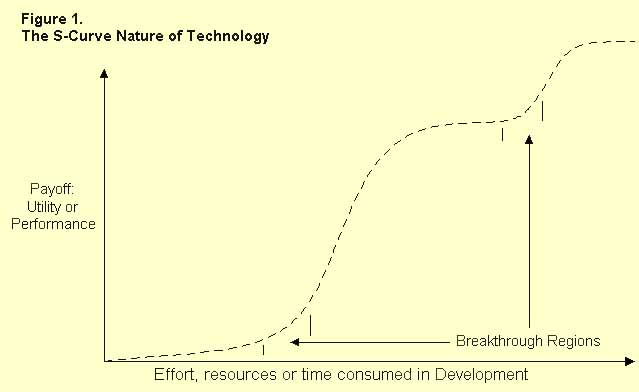
\includegraphics[width=\textwidth,height=\textheight,keepaspectratio]{./fig-1.jpg}
    \caption{The S-Curve Nature of Technology}
    \label{fig:S-Curve}
\end{figure}

To illustrate the S-curve concept, consider the development of aircraft, and in particular their speed. For many years after the Wright brothers, aircraft speeds crawled slowly forward. In 1940, they were still quite slow. Suddenly, each airplane designed was faster, until the limits of subsonic flight were reached. At that point, we were on a new S-curve. Again, the effort to reach transsonic flight consumed many resources and much time, but then the breakthrough was made. In a short time, aircraft were traveling at multiples of the speed of sound, at speeds nearly two orders of magnitude greater than those achieved shortly before World War II.\footnote{In common engineering parlance, an increase by an order of magnitude is approximately a tenfold increase. Astronomers, be wary.}

Note that the top of one S curve may -- in fact usually will -- be the base of another following it. Although the stream moves on inexorably, it is possible to exploit one or another aspect of technology at will. Which aspect to exploit will depend on several factors, the most important being your goals and your position on the S-curve.

Technology is interdependent: advances in one sector of technology soon influence areas which might naively have been believed unrelated. For example, the development of molecular chemistry techniques led to the art of microminiaturization, which allows development of computer technology beyond the expectations of only a few years ago. The revolution in computer sciences has made possible the development of on-board computers for missile guidance, and thus of accuracies not previously predicted. Increased accuracy has made possible the destruction of missile silos with much greater ease and smaller warheads.

Nuclear research, meanwhile, had developed smaller and lighter warheads; this coupled with increased accuracy has led to the development of Multiple Independently Targetable Re-Entry Vehicles (MIRV), each one of which uses on-board guidance computers. The increased kill capability stimulated research into silo hardening techniques, which led directly to what were called "hard rock silo" designs. That development made it possible to conduct certain mining operations that were previously financially infeasible. Examples of interdependence can be given without limit.\footnote{We should note that as part of the budget process to gather Congressional support, major programs such as Apollo and SDI had t identify "spinoffs" which can find application in the commercial world.} 

Thus, technology influences nearly every aspect of national life. In particular, technology influences strategy, forcing strategic revolutions at frequent intervals. There are those who say that strategy never changes. If they mean literally what they say, they have never appreciated the effects of the airplane and the ICBM, the possibilities for surprise attack created by these radical new weapons delivery systems coupled with thermonuclear explosives, and the effect they have on ground battles. If, however, they mean that the principles of strategy have not changed, they are more nearly correct, as we will discuss below.

The important fact is that technology paces strategy to a great extent, and forces the development of new military strategies which take the new technology into account. As we will show, it is dangerous to regard this relationship as one-sided. Technology and strategy are interrelated, and strategy can and should also pace technology.

This is well illustrated by the SDI program. President Reagan was convinced that the U.S. needed a new strategy. That strategy was impossible without new technology. His call for technology to make possible a strategy of 'assured survival' stimulated a dozen technology development programs. It is important to note that most of them worked, and some worked much better than we had supposed they would.

We have not always done badly in this race. Despite the opposition of a number of scientists, the feasibility and potentially decisive advantages of ballistic missiles were early recognized, and a program to develop and deploy these weapons was undertaken. The Thor IRBM was designed, developed, and ready to deploy in just over three years. Submarine launched missiles were developed in parallel. The IRBM was soon followed by the ICBM. Meanwhile, missile research led to capabilities in space technology.

Shortly before the first edition of this book was written, the major computer companies of the world decided that the United States would need no more than a dozen computers, none of them more powerful than the equipment that now sits on desktops in small businesses. The demands for further accuracy in missiles led to developments in miniaturization of components, including on-board guidance computers; the result became a full revolution in computer technology. That revolution's full extent cannot yet be measured.

Despite some spectacular successes, technology appears to many of our national leaders, and most of the Congress, to be an impersonal force. Although America is the leading technological power -- perhaps because we are the leading technological power -- many of our leaders do not really comprehend technology. As a consequence, technology remains largely a matter of individual initiative. Sometimes we do well. The first edition of this book contained lengthy analyses of our faults. Many have since been corrected.

Unfortunately, we still have no comprehensive strategy for winning the Technological War.

\section{The Decisive War}
The technological contest is a war. It is not a game against an impersonal force, it is a deadly conflict with an intelligent and implacable enemy. We do not suppose that a military commander who conducted his battles as they occurred, understanding neither the terrain nor the enemy and preparing only for the battle that he had already fought, would be properly performing his task. Yet, too often this is precisely what happens in the Technological War, which may be the most decisive engagement in the history of mankind. Technology has grown into the driving force, dictating to strategy; and strategy is conceived of as employment of systems already created by the technologists; that is, strategy is confined to operational decisions. This is akin to allowing the recruiting and supply officers to decide the conduct of a traditional land war.

The danger in the Technological War is that it is closely coupled with the Protracted Conflict, and a decisive lead in the Technological War can be converted into a decisive advantage in military weapons. Note that military power and technological power are coupled, but are not identical; military technology is not in and of itself a weapon system, but it can be used to create weapons systems. Thus a commanding lead in the Technological War can be achieved before a corresponding lead in military technology has been obtained.

As an example, the Soviet Union could, through the development of strategic nuclear defense technology, obtain a decisive lead in the Technological War at a time when the United States still possessed a clear superiority in deliverable weapons. This technology could then be used to create defense systems, and if the United States took no countermeasures during the deployment of those defensive systems, we would find ourselves in an inferior military position.

This is an especial danger if the numbers of strategic offensive weapons has been limited by arms reduction treaties and the Soviets then "break out" of the defensive and offensive limits imposed by the ABM Treaty and SALT. The closed nature of Soviet society makes planning for breakouts rather simple; the open nature of the US makes that nearly impossible. Note that the USSR used the breakout strategy following the 'gentleman's agreement' Test Ban.

During the 1970's the Soviet Union achieved (entirely predictable) spectacular gains in achievable accuracies, and also built large new missiles capable of carrying a dozen and more warheads over intercontinental distances. The United States relied on Arms Control negotiations for security; when these failed, we found ourselves facing a "window of vulnerability" -- that is, a period of time during which, if we do not act promptly and intelligently, the Soviet Union could construct a first strike capability. The Soviets continued to deploy ICBM's in large numbers. The "window of vulnerability" has not entirely been overcome as of 1988, although President Reagan's strategic force modernization program took away much of the danger.

\textit{glasnost} and \textit{perestroika} promise a new era in strategic conflict; they have not eliminated the technological war.

In addition, the USSR has undertaken serious research into strategic defense systems, not merely building on the single system permitted under the ABM Treaty, but also investigating entirely new concepts. When the US began its own strategic defense investigation in 1983, the Soviet Union redoubled its efforts, including construction of large components such as the radar system at Krasnyarsk.

None of this was decisive. Victory in the Technological War is achieved when a finite game participant (ie, one who wishes to bring the game to an end by winning it) has a technological lead so far advanced that his opponent cannot overcome it until after the leader has converted his technology into decisive weapons systems. The loser may know that he has lost, and know it for quite a long time, yet be unable to do anything about it. To continue the above example, if the Soviet Union were able to develop the technology in time to deploy ballistic missile defense systems of his own before ours could be installed and operational, we would be beaten, even though the U.S.S.R. might spend several years in deployment of his own system. Our only choices would be the development of a penetration system that his defenses could not counter (such as manned bombers of very high capabilities)\footnote{We would, of course, have not only to invent and develop these bombers but build them in quantity, fly them, train the pilots, etc., and do it all within the time limits of U.S.S.R. deployment.}, surrender, or preventive war.

Now, in the late 1980's, many believe that development of space laser battle stations will be a decisive move in the technological war. The laser battle station could, at least in theory, destroy an entire ICBM force in flight, then burn down the enemy's bomber fleet for encore. Such a station once in place could give a decisive lead to its owner.

In practice a space laser battle station would require auxiliary equipment for its own defense, since there are many ways to attack such a system; on the other hand, it is likely that such escort systems would be deployed by any power constructing a large space laser battle station.

The Soviets have raised the specter that other space weapons which they call "space strike weapons" are being developed as part of the US Strategic Defense Initiative. The fact that the Soviets emphasize such a threat at a time when the US has no concepts, let alone a technology which could produce them, raises the concern that the Soviets are developing them, because the Soviets often accuse the US of developing and deploying weapons which they themselves are developing.

Several years after the initial Soviet assertions that SDI raised the spectre of such weapons, the Soviets defined them for Ambassador Henry Cooper, head of the US negotiating team on defense and space talks, as : 1) Ground to space weapons, 2) Space to space weapons; and 3) Space to ground weapons. The U.S.S.R. has demonstrated all three: Galosh interceptors against satellites; co-orbital ASATs; and FOBs, which are bombs in orbit.

If space and ground based ICBM defenses could give us a decisive advantage, they would confer no less advantage on the Soviets if we allow our enemies to develop them without any counter on our part.

This is the unique feature of the Technological War. Military superiority or even supremacy is not permanent, and never ends the conflict unless it is used. The United States considers the Technological War as an infinite game: one which is not played out to a decisive victory. We are committed to a grand strategy of defense, and will never employ a decisive advantage to end the conflict by destroying our enemies. Consequently, we must maintain not only military superiority but technological supremacy. \textbf{The race is an alternative to destructive war, not the cause of military conflict.}

In summary, proper conduct of the Technological War requires that strategy drive technology most forcefully; that there be an overall strategy of the Technological War, allocating resources according to well-defined objectives and an operational plan, not merely strategic elements which make operational use of the products of technology. Instead of the supply officer and the munitions designer controlling the conduct of this decisive war, command must be placed in the hands of those who understand the Technological War; and this requires that they first understand the nature of war.

Lest the reader be confused, we do not advocate that the Technological War be given over to the control of the scientists, or that scientists should somehow create a strategy of technological development. We mean that an understanding of the art of war is more important than familiarity with one or another of the specialties of technology. It is a rare scientist who makes a good strategist; and the generals of the Technological War need not be scientists any more than the generals of the past needed to be good riflemen or railroad engineers.

Like all wars, the Technological War must be conducted by a commander who operates with a strategy. It is precisely the lack of such a strategy that brought the United States to the 1970's low point in prestige and power, with her ships seized across the world, her Strategic Offensive Forces (SOF) threatened by the growing Soviet SOF -- and with the United States perplexed by as simple a question as whether to attempt to defend her people from enemy thermonuclear bombs, and unable to win a lesser war in South East Asia.\footnote{Since this book is intended to be a discussion of principles, not of current specific problems, it may be well in print long after the present war in Vietnam is ended. We venture to predict, however, that for many years after this is written (1970) there will be wars in Asia, including South East Asia and the area formerly known as Indo-China, and their outcomes will be of concern to the United States.}

We had neither generals nor strategy, and muddled through the most decisive conflict in our national history.

Much of this changed in 1981. President Reagan's 1983 call for SDI was in response to strategic analyses presented by General Daniel O. Graham and others.

There always were exceptions to this unsatisfactory record of American performance. General Bernard Schriever created a military organization for strategic analysis which was responsible for our early commanding lead over the Soviets in ballistic missiles, despite the fact that the U.S. had allowed the U.S.S.R. many years' head start in missile development after World War II.\footnote{The authors recall the frustration of Wernher Von Braun and other rocketry experts when the last of the V-2 rockets brought to the United States were used, not for the development of rocket sciences, but as supersonic test beds for aircraft parts to avoid spending the funds required for construction of supersonic wind tunnels. This retarded the development of both missiles and supersonic aircraft, of course.} The Air Force's Project Forecast and later Project 75, was an attempt to let strategy react to, then drive, technology; these, too, were creations of General Schriever's.

In the Navy there have also been notable attempts to allow strategy to influence technology and produce truly modern weapons systems.

\section{The Elements of Strategy}
\subsection{What is Strategy}
Because there seems to be little understanding of strategy and its effect on the Technological War, we will briefly review some general principles of strategy and warfare. Our purpose is not to teach the elements of strategy, which would require another book, but rather to make the reader aware of strategy and some of its complexities.

According to the traditional concept of military strategy it should mean the art of employing military forces to achieve the ends set by political policy. This definition was formulated by [Sir Basil Henry] Liddell Hart in 1929 and it hardly differs from that of Clausewitz. Raymond Aron follows it almost word for word. France's leading strategist of the 60's commented:

"In my view this definition is too restrictive because it deals with military forces only. I would put it as follows: the art of applying force so that it makes the most effective contribution towards achieving the ends set by political policy...

"In my view the essence of strategy is the abstract interplay which, to use Foch's phrase, springs from the clash between two opposing wills. It is the art which enables a man, no matter what the techniques employed, to master the problems set by any clash between two opposing wills. It is the art which enables a man, no matter what the techniques employed, to master the problems set by any clash of wills and as a result to employ the techniques available with maximum efficiency. it is therefore the art of the dialectic of force, or, more precisely, the art of the dialectic of two opposing wills using force to resolve their dispute.\footnote{General d'Armee Andre Beaufre, Introduction to Strategy (New York: Praeger, 1965), p. 22.}

In our judgment it would be hard to better the above definition provided that we understand force to include the broader concept of power and force. Examining the definition shows us several important aspects of the Technological War and its strategy.

First, we see that strategy involves two opposing wills. This in itself sets the Technological War apart from the simple development of technology. The development of technology is a game against nature, which may be uncooperative, but which never deceives or actively conspires to prevent your success. The Technology War is a contest with an intelligent opponent who seeks to divert you from seeing his purpose, and to surprise you with his results.

Secondly, strategy involves the use of power and force. In the Technological War, the more power is extant, the less often force needs to be used in the primary or decisive mode of the conflict. In the place of battles, the Technological War general disposes his own resources so as to maximize the power he holds and at the same time compel the enemy to make maximum dispersal of his. To make the enemy counter each move you make, and dance to your tune, is the aim of a Technological War strategy. In the ideal, if the enemy were required continually to build purely defensive weapons which might protect him from your weapons but could not possibly harm you, you could be said to have won a major engagement in the Technological War. In the contest between wills, seizing and holding the initiative is of importance; as indeed it has been for a long, long time:

You hear that Phillip is in the Chersonese, and you vote an expedition there; you hear that he is in Thessaly, and you vote one there. You march the length and breadth of Greece at his invitation, and you take your marching orders from him.\footnote{Demosthenes, First Phillipic to the People of Athens}

But if the power ratio is ambiguous, the decision as to who is the stronger will be made by force, which is the application of power in battle. Other things being equal, battles are won by superior technology. But clearly superior technology prevents battle.

\section{The Principles of War}
War is an art; it is not an exact science, although the Soviet Union considers it to be so. Precisely because there is an intelligent opponent, there are real uncertainties about war, not merely statistical uncertainties which may be measurable. Every attempt to reduce war to an exact science has ended in a dismal failure. The advent of the computer and systems analysis, useful as both may be, has not changed this fact, although it has often been forgotten.

Part of the traditional method of learning the art of war is studying the principles of war. These principles are a set of general concepts, like holds in wrestling, and no exact group of principles is universally recognized. Some strategists combine several into one or divide one of those we show into several. The following list will serve well enough for our purpose:

\begin{itemize}
    \item The Principle of the Objective
    \item The Principle of the Initiative
    \item The Principle of Surprise
    \item The Principle of the Unity of Command
    \item The Principle of Mass (Concentration of Force)
    \item The Principle of Economy of Forces
    \item The Principle of Mobility
    \item The Principle of Security
    \item The Principle of Pursuit
\end{itemize}

It will be noted that some of these principles, if carried to their extremes, would be contradictory. They are intended to serve not as a formula for the planning of a battle, but rather as a set of guides or a checklist which the planner ignores only with peril. They are as applicable to the Technological War as to any other war. At first glance, it might seem that one principle or another might be more directly applicable to the Technological War than the others, but in fact none can be disregarded if success is to be achieved. We will have occasion to refer to them from time to time in the analysis below.

\section{Strategy and Technology}
The United States today has no technological strategy as we define it. However, as the philosophers have noted, "Everyone has a metaphysics, including those who deny it." The same applies to a technological strategy.

Instead of an integrated strategy of technology, we have a series of independent and often uncorrelated decisions on specific problems of technology. This is hardly a strategy. A technological strategy would involve the setting of national goals and objectives by political leaders; it would be integrated with other aspects of our national strategy, both military and nonmilitary (Initiative, Objective, and Unity of Command); it would include a broad plan for conducting the Technological War that provided for surprising the enemy, pursuing our advantage (Pursuit), guarding against being surprised (Security), allocating resources effectively (Economy of Forces), setting milestones and building the technological base (Objective), and so forth. Lesser conflicts such as that in Vietnam would be governed by a broad strategic doctrine instead of being considered isolated and treated as crises.

In our national strategy, far too much attention has been given to current affairs and to specific conflict situations at particular times and places. There has been no serious attempt to integrate the individual decisions, or relate them to a comprehensive grand strategy that is adequate to overcome the challenges. The few attempts we have made to manage technological decisions properly were disastrous; examples are the ludicrous "saving" achieved through the TFX and the equally dismal saving through over-management of the C5A program. We have confused a strategy of technology with centralized interference in the design or production of specific weapons and the imposition of a "standard management plan".

Micromanagement, whether by Congress or the Pentagon, is no substitute for a genuine strategy.

The results of our neglecting technological strategy are easily seen. Our performance in Vietnam was disastrous. We failed to exploit our superior technology to grasp a commanding lead in either inner space or outer space. Our merchant marine where it exists at all flies the proud flag of Panama or Liberia. Meanwhile, many of our young men are sent to fight overseas with weapons that make use of principles discovered by Roger Bacon in the thirteenth century.

\begin{mdframed}[backgroundcolor=black!10]
Alas, we see no reason to revise the above after over twenty years. Our failure to understand what the Viet Nam War was about cost us all the blood and treasure we had previously invested; the Soviets have surpassed us in manned space exploitation and ICBM deployment, and are keeping up in missile defense technology; and we were unable to use our technology or military power in the Iranian hostage crisis.
Our attempts to remedy this situation have generally made things worse. Endless reviews and meaningless analyses have driven lead times to inordinate lengths. Whereas in 1941-44 we were able to conceive, design, build, and deploy large numbers of new military aircraft within three years, this is inconceivable today (1991).
\end{mdframed}

The reasons for this dismal performance are complex; it is not necessary to understand all of them and it is not germane to blame anyone. Events caught up with us, the stream of technology swept us along, and only recently did we begin to realize the nature of the Technological War. In fact, one reason we have no strategy of technology is that not everyone realizes we are at war; but perhaps the most important reason is the basic failure to understand the nature of technology itself, and particularly the problems of lead time which produce a crisis-oriented design process.

Our opponents created crises, and we have had to meet them. Decision makers at the national level concentrate on fighting today's fire, partly because they hope that the current trouble will be the last but mostly because of the long lead time involved in technology. A President called upon to spend money in any fiscal year actually is spending money to solve the problems of a President two terms later. But even if we try to find comfort in expenditures for research and development, we must understand that these are oriented to specific projects and tasks and do not result from technological strategy.

\begin{mdframed}[backgroundcolor=black!10]
During the 1970's, the expenditures in research and development were cut back; the result was that high technology exports became less valuable than agriculture in our balance of payments. SDI refocussed U.S. efforts and halted what had been a continuous erosion of our technological base. Fortunately the Soviets have their problems too, caused by their generally bad management practices; but do note that the Soviet military economy is run on an entirely different basis from their notoriously inefficient civilian economy. Meanwhile, as the Soviet threat to Europe abates, the Technological War does not, for many of our erstwhile allies, now freed from fear of the Soviets, can put even more of their resources into that war -- and we have yet to examine the potential of Eastern Europe.
\end{mdframed}

Our misunderstanding of the Technological War is illustrated by our failure to build an organization for conducting technological warfare. The review of the annual budget and of individual projects in basic research, in applied research, in development, and in procurement is the only process by which our technological development is controlled directly. Other influences such as the statements of requirements and the evaluation of military worth are felt only at the level of individual projects. Overall evaluation of the research and development effort and of its relations to strategy is rudimentary.

An example of how irrelevant factors influence our efforts, and perhaps one of the decisive signs of the times: the January 20, 1969 issue of Aviation Week and Space Technology, the most influential journal in the aerospace field, included a report entitled "Viet Lull Advances New Weapons". The article makes clear that the budgetary funding level of many advanced new weapons systems, including research and development, basic technology, and actual system procurement, is largely dependent on the continuation of a "lull" in the Vietnam war. Given a proper strategy for the Technological War and proper command of our efforts, the title should read "Advanced New Weapons End Vietnam War".

\subsection{1988}
Perhaps the most glaring examples of our failure to grasp the fundamentals of a technological strategy are found in our failure to build on the Apollo program to create a space station and build systems for rapid and assured access to the space environment; to develop defenses against ballistic missiles; and to make the transition from aerospace power to space power. Such failures are clear illustrations of that a strategy of technology should be. The goal of this book is to try to prevent future errors of this kind.

\subsection{1997}
We cannot emphasize this too strongly. The Seventy Years War which began in St. Petersburg in 1917 effectively came to an end with the destruction of the Berlin Wall, leaving the United States of America as the only Superpower. Victory in the Seventy Years War, sometimes (in our judgment mistakenly) called The Cold War, did not bring "the end of history" as was naively prophesied by Francis Fukuyama and others.

Fukuyama's thesis was that with the end of the Cold War all nations would now embrace liberal democracy; and liberal democracies do not make war on each other. Therefore, while mankind would now prevail, there would be no more history, which is the record of change, often by violence.

By now it should be clear that all the nations of the Earth have not embraced liberal democracy. It is not inevitable that the United States itself will be governed by what we understand as liberal democracy much beyond the end of this Millenium. Being the only Superpower carries with it the danger of a fundamental transformation from democracy to Empire, and there are powerful forces pushing the United States toward Imperium if not Empire. In any event, there are plenty of regimes motivated by religious fervor, nationalism and tribalism, and ruled by elites or dictators.

The end of the Seventy Years War has not brought lasting peace, nor has it ended the Technological War; indeed, the stakes are now much higher, and the price of entry into the Technological War is far lower; with only one Superpower in the game, a potential Superpower has only one competitor, and that a somewhat complacent one that cannot believe anyone can possibly catch up.

Unfortunately, catching up is quite possible. Just as the threat of a strategic sidestep into space negated much of the USSR's vast missile establishment and threatened the USSR with economic ruin, a real move into space--a real conquest of the High Frontier, if you will--would put the United States in a vulnerable position.

This is not the place to generate scenarios of potential conflicts over the next fifty years; suffice it to say that there remain a number of powers with unsatisfied ambitions and both territorial and economic claims. Some, like China and Indonesia have large populations, an educated elite, high industrial potential, and no great experience with, or desire for, liberal democracy.

The world remains a dangerous place, and a Strategy of Technology remains the most prudent course for the United States; and it is a course we are not properly following.
